\begin{abox}
	Net-2019 
\end{abox}
\begin{enumerate}
	\item In a bacterial cell, a protein is synthesized at random location in the cytoplasm. The protein has to reach one pole of the cell for its appropriate function. The protein reaches the pole by
	 \begin{tasks}(2)
		\task[\textbf{a.}]Chemical attraction
		\task[\textbf{b.}]Random movement
		\task[\textbf{c.}]Enzymatic action
		\task[\textbf{d.}] Attraction between opposite charges
	\end{tasks}
	\item A precious stone breaks into four pieces having weights in the proportion $1: 2: 3: 4$. The value of such a stone is proportional to the square of its weight. What is the percent loss in the value incurred due to breaking?
	 \begin{tasks}(4)
		\task[\textbf{a.}]0
		\task[\textbf{b.}]30
		\task[\textbf{c.}]70
		\task[\textbf{d.}] 90
	\end{tasks}
	\item Two runners starting together run on a circular path taking 6 and 8 minutes, respectively, to complete one round. How many minutes later do they meet again for the first time on the start line, assuming constant speeds
	 \begin{tasks}(4)
		\task[\textbf{a.}]8
		\task[\textbf{b.}]24
		\task[\textbf{c.}]32
		\task[\textbf{d.}] 60
	\end{tasks}
	\item 	 The distribution of grades secured by students in a class is given in the table below.\\\\
	\begin{tabular}{|c|c|}
		\hline Grade & Fraction of the Population \\
		\hline A & $0.1$ \\
		\hline B & $0.4$ \\
		\hline C & $0.3$ \\
		\hline D & $0.2$ \\
		\hline
	\end{tabular}\\\\
	What is the least possible population of the class?
	 \begin{tasks}(4)
		\task[\textbf{a.}]2
		\task[\textbf{b.}]4
		\task[\textbf{c.}]8
		\task[\textbf{d.}] 10
	\end{tasks}
\item  The nine numbers $x_{1}, x_{2}, x_{3} \ldots x_{9}$, are in ascending order. Their average $m$ is strictly greater than all the first eight numbers. Which of the following is true?
	(a) Average $\left(x_{1}, x_{2} \ldots x_{9}, m\right)>m$ and Average $\left(x_{2}, x_{3}, \ldots x_{9}\right)>m$
	(b) Average $\left(x_{1}, x_{2} \ldots x_{9}, m\right)<m$ and Average $\left(x_{2}, x_{3}, \ldots x_{9}\right)<m$
	(c) Average $\left(x_{1}, x_{2} \ldots x_{9}, m\right)=m$ and Average $\left(x_{2}, x_{3}, \ldots x_{9}\right)>m$
	(d) Average $\left(x_{1}, x_{2} \ldots x_{9}, m\right)<m$ and Average $\left(x_{2}, x_{3}, \ldots x_{9}\right)=m$
\item  Which among the following diagrams represents women, mothers, human beings?
	 \begin{tasks}(2)
		\task[\textbf{a.}]
		\begin{figure}[H]
			\centering
			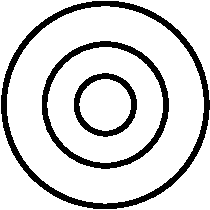
\includegraphics[height=2cm,width=2cm]{Net-19-1}
		\end{figure}
		\task[\textbf{b.}]
		\begin{figure}[H]
			\centering
			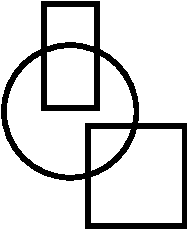
\includegraphics[height=2.4cm,width=2cm]{Net-19-2}
		\end{figure}
		\task[\textbf{c.}]
		\begin{figure}[H]
			\centering
			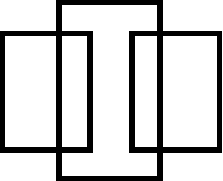
\includegraphics[height=2cm,width=2cm]{Net-19-3}
		\end{figure}
		\task[\textbf{d.}] 
		\begin{figure}[H]
			\centering
			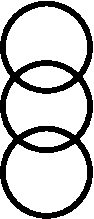
\includegraphics[height=2.3cm,width=1cm]{Net-19-4}
		\end{figure}
	\end{tasks}
\item  A boy and a girl make the following statements, of which at most one is correct:
The one in a white shirt says: "I am a girl" (statement - I)
The one in a blue shirt says: "I am a boy" (statement - II)
Which of the following is the correct inference?
	 \begin{tasks}(1)
		\task[\textbf{a.}]Statement - I is correct but statement - II is incorrect
		\task[\textbf{b.}]Statement - II is correct but statement - I is incorrect
		\task[\textbf{c.}]Both statement I and II are incorrect
		\task[\textbf{d.}] The correctness of the statements I and II cannot be ascertained	
	\end{tasks}
\item  How many quadrilaterals does the following figure have?	
\begin{figure}[H]
	\centering
	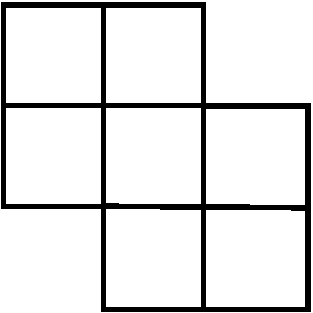
\includegraphics[height=3cm,width=3cm]{Net-19-5}
\end{figure}
 \begin{tasks}(4)
	\task[\textbf{a.}]17
	\task[\textbf{b.}]18
	\task[\textbf{c.}]19
	\task[\textbf{d.}] 20
\end{tasks}
\item  12 balls, 3 each of the colours red, green, blue and yellow are put in a box and mixed. If 3 balls are picked at random, without replacement, the probability that all 3 balls are of the same colour is
 \begin{tasks}(4)
	\task[\textbf{a.}]$\frac{1}{4}$
	\task[\textbf{b.}] $\frac{1}{12}$
	\task[\textbf{c.}]$\frac{1}{36}$
	\task[\textbf{d.}]$\frac{1}{55}$ 
\end{tasks}
\item  Some aliens observe that roosters call before sunrise every day. Having no other information about roosters and sunrises, which of the following inferences would NOT be valid?
 \begin{tasks}(1)
	\task[\textbf{a.}]Rooster-call and sunrise may be independent cyclic events with the same periodicity
	\task[\textbf{b.}]Both may be triggered by a common cause
	\task[\textbf{c.}]Rooster-call may be causing the sunrise
	\task[\textbf{d.}]Sunrise cannot be the cause of rooster call as the rooster-call precedes sunrise 
\end{tasks}
\item  Twenty-one litres of water in a tank is to be divided into three equal parts using only 5,8 and 12 litre capacity cans. The minimum number of transfers needed to achieve this is
 \begin{tasks}(4)
	\task[\textbf{a.}]3
	\task[\textbf{b.}]4
	\task[\textbf{c.}]5
	\task[\textbf{d.}] 7
\end{tasks}
\item  Of four agents Alpha, Beta, Gamma and Delta, three have to be sent together on a mission. If Alpha and Beta cannot go together, Beta and Gamma cannot go together and Gamma and Delta cannot go together, then which of the following holds?
 \begin{tasks}(1)
	\task[\textbf{a.}]Any three agents can be sent.
	\task[\textbf{b.}]Alpha, Delta and any one out of Beta and Gamma can be sent
	\task[\textbf{c.}] Beta, Gamma and any one out of Alpha and Delta can be sent
	\task[\textbf{d.}] The mission is impossible.
\end{tasks}
\item  An open rectangular box is made by excluding the four identical corners of a piece of paper as shown in the diagram and folding it along the dotted lines
\begin{figure}[H]
	\centering
	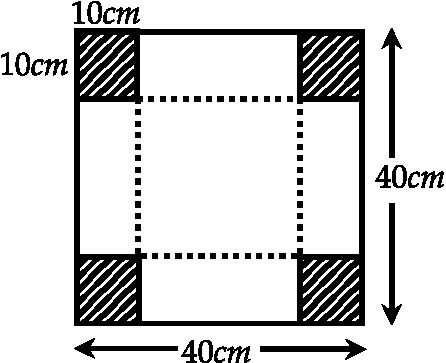
\includegraphics[height=3.1cm,width=4cm]{Net-19-6}
\end{figure}
The capacity of the box $\left(\mathrm{in} \mathrm{cm}^{3}\right)$ is
 \begin{tasks}(4)
	\task[\textbf{a.}] 8000
	\task[\textbf{b.}]1000
	\task[\textbf{c.}]4000
	\task[\textbf{d.}] 6000
\end{tasks}
\item  Which of the following is the largest?
$
2^{50}, 3^{40}, 4^{30}, 5^{20}
$
 \begin{tasks}(4)
	\task[\textbf{a.}] $2^{50}$
	\task[\textbf{b.}]$3^{40}$
	\task[\textbf{c.}]$4^{30}$
	\task[\textbf{d.}]$5^{20}$ 
\end{tasks}
\item  A monkey climbs a tree to eat fruits. The amount of energy gained from eating fruits and the energy spent in climbing on different branches have a relationship shown in the figure.
\begin{figure}[H]
	\centering
	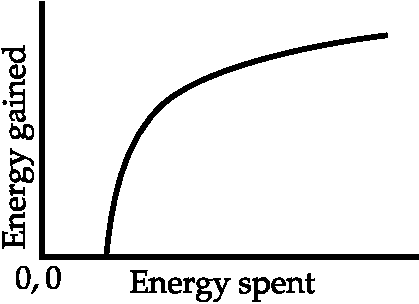
\includegraphics[height=2cm,width=3cm]{Net-19-7}
\end{figure}
The ratio of energy gained to energy spent will be the maximum
 \begin{tasks}(1)
	\task[\textbf{a.}] At a point where the slope of the curve is the maximum
	\task[\textbf{b.}] At a point where the slope of the curve is unity
	\task[\textbf{c.}]At a point on the curve where the tangent passes through the origin
	\task[\textbf{d.}] At the highest point on the curve
\end{tasks}
\item  The length of a cylinder is measured 10 times yielding 10 distinct values. For this set of values, consider the following statements\\
A. Five of these values will lie above the mean and five below it\\
B. Five of these values will lie above median and five below it\\
C. At least one value will lie above the mean\\
D. At least one value will lie at the median\\
Which of the statements are necessarily correct?
 \begin{tasks}(4)
	\task[\textbf{a.}] $\mathrm{B}$ and $\mathrm{C}$
	\task[\textbf{b.}] $\mathrm{A}$ and $\mathrm{C}$
	\task[\textbf{c.}] B and D
	\task[\textbf{d.}]$\mathrm{A}, \mathrm{C}$ and $\mathrm{D}$ 
\end{tasks}
\item  In the given circle, $O$ is the centre, $\angle P A O=40^{\circ}, \angle P B Q=30^{\circ}$ and outer angle
$$
\angle A O B=220^{\circ} \text {. }
$$
Then $\angle A Q B$ is
\begin{figure}[H]
	\centering
	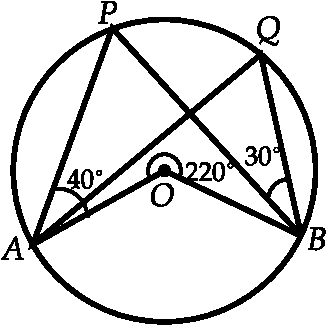
\includegraphics[height=3cm,width=3cm]{Net-19-8}
\end{figure}
 \begin{tasks}(4)
	\task[\textbf{a.}] $70^{\circ}$
	\task[\textbf{b.}] $80^{\circ}$
	\task[\textbf{c.}]$60^{\circ}$
	\task[\textbf{d.}] $110^{\circ}$
\end{tasks}
\item  A canal system is shown in the figure
\begin{figure}[H]
	\centering
	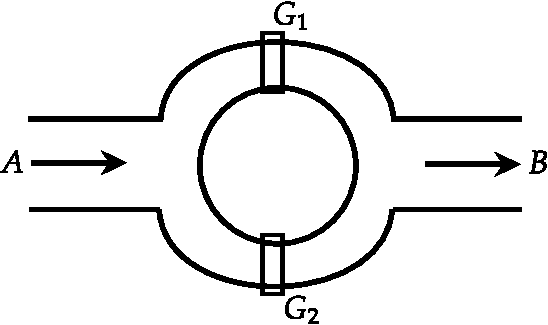
\includegraphics[height=2cm,width=3.5cm]{Net-19-9}
\end{figure}
Water flows from $A$ to $B$ through two channels. Gates $G_{1}$ and $G_{2}$, are operated independently to regulate the flow. Probability of $G_{1}$ to be open is $10 \%$ while that of $G_{2}$ is $20 \%$. The probability that water will flow from $A$ to $B$ is
 \begin{tasks}(4)
	\task[\textbf{a.}]$10 \%$
	\task[\textbf{b.}]$20 \%$
	\task[\textbf{c.}]$28 \%$
	\task[\textbf{d.}]$30 \%$
\end{tasks}
\item  A long ream of paper of thickness $t$ is rolled tightly. As the roll becomes larger, the length of the paper wrapped in one turn exceeds the length in the previous turn by
 \begin{tasks}(4)
	\task[\textbf{a.}]$t$
	\task[\textbf{b.}]$2 t$
	\task[\textbf{c.}]$\pi t$
	\task[\textbf{d.}] $2 \pi t$
\end{tasks}
 \item   Point $A$ on a wheel of radius $r$ touches the horizontal plane at point $P$. It rolls without slipping, till point $A$ is at the highest position in the first turn. What is the final distance $A P$ ?
 \begin{figure}[H]
 	\centering
 	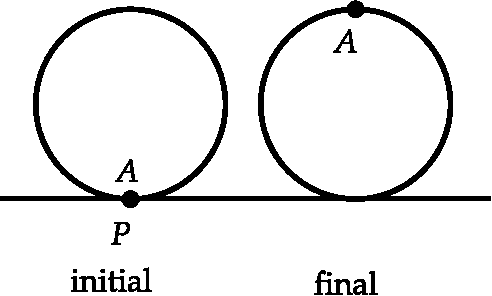
\includegraphics[height=2cm,width=3.5cm]{Net-19-10}
 \end{figure}
 \begin{tasks}(2)
	\task[\textbf{a.}]$2 r$
	\task[\textbf{b.}]$r \sqrt{\left(1+\pi^{2}\right)}$
	\task[\textbf{c.}] $r \sqrt{\left(4+\pi^{2}\right)}$
	\task[\textbf{d.}] $2 r \sqrt{\left(1+\pi^{2}\right)}$
\end{tasks}
\item  An object is dropped on a cushion from a height $10 \mathrm{~m}$ above it. On being hit, the cushion is depressed by $0.1 \mathrm{~m}$. Assuming that the cushion provides a constant resistive force, the deceleration of the object after hitting the cushion, in terms of the acceleration due to gravity $g$ is
 \begin{tasks}(4)
	\task[\textbf{a.}]$10 g$
	\task[\textbf{b.}] $50 \mathrm{~g}$
	\task[\textbf{c.}] $100 \mathrm{~g}$
	\task[\textbf{d.}]  $g$
\end{tasks}
\item  A turn-table is rotating with a constant angular velocity $\omega_{0}$. In the rotating frame fixed to the turntable, a particle moves radially outwards at a constant speed $v_{0}$. The acceleration of the particle in the $r \theta$ coordinates, as seen from an inertial frame, the origin of which is at the centre of the turntable, is
 \begin{tasks}(2)
	\task[\textbf{a.}]$-r \omega_{0}^{2} \hat{r}$
	\task[\textbf{b.}]$2 r \omega_{0}^{2} \hat{r}+v_{0} \omega_{0} \hat{\theta}$
	\task[\textbf{c.}]$r \omega_{0}^{2} \hat{r}+2 v_{0} \omega_{0} \hat{\theta}$
	\task[\textbf{d.}] $-r \omega_{0}^{2} \hat{r}+2 v_{0} \omega_{0} \hat{\theta}$
\end{tasks}
\item  Assume that the earth revolves in a circular orbit around the sun. Suppose the gravitational constant $G$ varies slowly as a function of time. In particular, it decreases to half its initial value in the course of one million years. Then during this time the
(a) Radius of the earth's orbit will increase by a factor of two
(b) Total energy of the earth remains constant
(c) Orbital angular momentum of the earth will increase
(d) Radius of the earth's orbit remains the same.
\item  A particle of mass $m$ moves in One dimension in the potential $V(x)=k x^{4},(k>0)$. At time $t=0$ the particle starts from rest at $x=A$.
For bounded motion, the time period of its motion is
 \begin{tasks}(2)
	\task[\textbf{a.}]Proportional to $A^{-1 / 2}$
	\task[\textbf{b.}]Proportional to $A^{-1}$
	\task[\textbf{c.}] Independent of $A$
	\task[\textbf{d.}]  Not well-defined (the system is chaotic)
\end{tasks}
\item  The infinite square-well potential of a particle in a box of size a is modified as shown in the figure below (assume $\Delta<<a$ )
\begin{figure}[H]
	\centering
	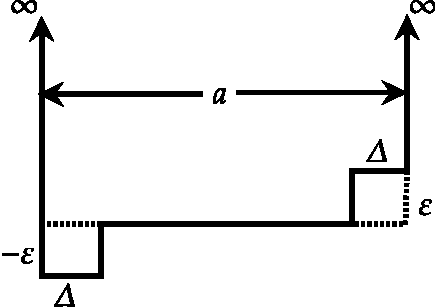
\includegraphics[height=2.7cm,width=3.5cm]{Net-19-11}
	\caption{}
	\label{}
\end{figure}
The energy of the ground state, compared to the ground state energy before the perturbation was added
 \begin{tasks}(2)
	\task[\textbf{a.}]Increases by a team of order $\varepsilon$
	\task[\textbf{b.}] Decreases by a term of order $\varepsilon$
	\task[\textbf{c.}]Increases by a term of order $\varepsilon^{2}$
	\task[\textbf{d.}]  Decreases by a term of order $\varepsilon^{2}$
\end{tasks}
\item  A quantum particle of mass $m$ in one dimension, confined to a rigid box as shown in the figure, is in its ground state. An infinitesimally thin wall is very slowly raised to infinity at the centre of the box, in such a way that the system remains in its ground state at all times. Assuming that no energy is lost in raising the wall, the work done on the system when the wall is fully raised, eventually separating the original box into two compartments, is
\begin{figure}[H]
	\centering
	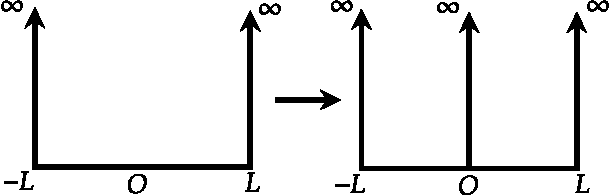
\includegraphics[height=2cm,width=6cm]{Net-19-12}
\end{figure}
 \begin{tasks}(2)
	\task[\textbf{a.}]$\frac{3 \pi^{2} \hbar^{2}}{8 m L^{2}}$
	\task[\textbf{b.}]$\frac{\pi^{2} \hbar^{2}}{8 m L^{2}}$
	\task[\textbf{c.}] $\frac{\pi^{2} \hbar^{2}}{2 m L^{2}}$
	\task[\textbf{d.}] 0
\end{tasks}
\item  The wavefunction of a free particle of mass $m$, constrained to move in the interval $-L \leq x \leq L$, is $\psi(x)=A(L+x)(L-x)$, where $A$ is the normalization constant. The probability that the particle will be found to have the energy $\frac{\pi^{2} \hbar^{2}}{2 m L^{2}}$ is
 \begin{tasks}(2)
	\task[\textbf{a.}]0
	\task[\textbf{b.}]$\frac{1}{\sqrt{2}}$
	\task[\textbf{c.}]$\frac{1}{2 \sqrt{3}}$
	\task[\textbf{d.}] $\frac{1}{\pi}$ 
\end{tasks}
\item  A particle moving in a central potential is described by a wavefunction $\psi(r)=z f(r)$ where $r=(x, y, z)$ is the position vector of the particle and $f(r)$ is a function of $r=|r|$.
If $L$ is the total angular momentum of the particle, the value of $L^{2}$ must be
 \begin{tasks}(2)
	\task[\textbf{a.}]$2 \hbar^{2}$
	\task[\textbf{b.}]$\hbar^{2}$
	\task[\textbf{c.}]$4 \hbar^{2}$
	\task[\textbf{d.}]$\frac{3}{4} \hbar^{2}$ 
\end{tasks}
\item  A particle of mass in and energy $E>0$. in one dimension is scattered by the potential below.
\begin{figure}[H]
	\centering
	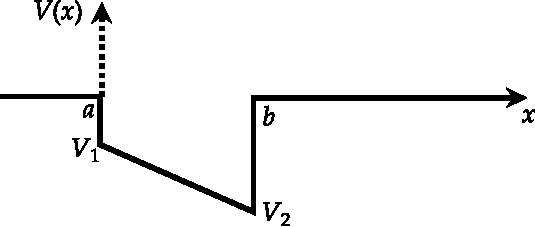
\includegraphics[height=2.3cm,width=5cm]{Net-19-13}
\end{figure}
If the particle was moving from $x=-\infty$ to $x=\infty$, which of the following graphs gives the best qualitative representation of the wavefunction of this particle?
 \begin{tasks}(2)
	\task[\textbf{a.}]
	\begin{figure}[H]
		\centering
		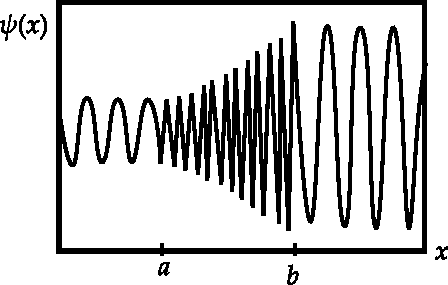
\includegraphics[height=3cm,width=5cm]{Net-19-14}
	\end{figure}
	\task[\textbf{b.}]
		\begin{figure}[H]
		\centering
		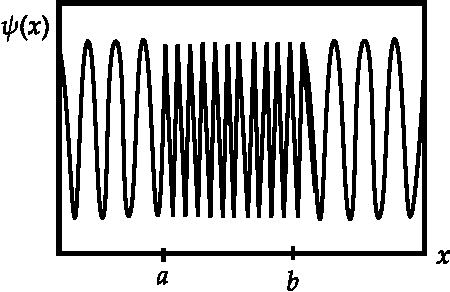
\includegraphics[height=3cm,width=5cm]{Net-19-15}
	\end{figure}
	\task[\textbf{c.}]
		\begin{figure}[H]
		\centering
		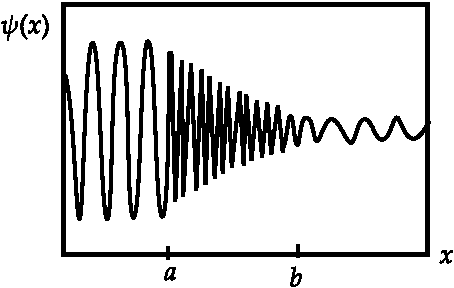
\includegraphics[height=3cm,width=5cm]{Net-19-16}
	\end{figure}
	\task[\textbf{d.}] 
		\begin{figure}[H]
		\centering
		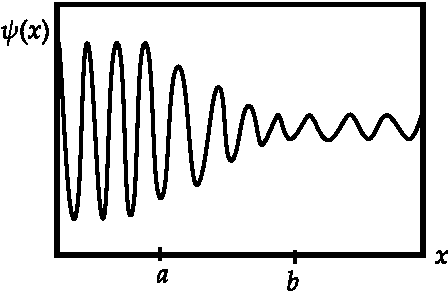
\includegraphics[height=3cm,width=5cm]{Net-19-17}
	\end{figure}
\end{tasks}
\item  Consider a planar wire loop as an $n$-sided regular polygon, in which $R$ is the distance from the centre to a vertex. If a steady current $I$ flows through the wire, the magnitude of the magnetic field at the centre of the Loop is
 \begin{tasks}(2)
	\task[\textbf{a.}]$\frac{\mu_{0} I}{2 R} \sin \left(\frac{2 \pi}{n}\right)$
	\task[\textbf{b.}] $\frac{\mu_{0} n I}{4 \pi R} \sin \left(\frac{\pi}{n}\right)$
	\task[\textbf{c.}]$\frac{\mu_{0} n I}{2 \pi R} \tan \left(\frac{2 \pi}{n}\right)$
	\task[\textbf{d.}] $\frac{\mu_{0} n I}{2 \pi R} \tan \left(\frac{\pi}{n}\right)$
\end{tasks}
\item  Two coherent plane electromagnetic waves of wavelength $0.5 \mu \mathrm{m}$ (both have the same amplitude and are linearly polarized along the $z$-direction) fall on the $y=0$ plane. Their wave vectors $k_{1}$ and $k_{1}$ are as shown in the figure
\begin{figure}[H]
	\centering
	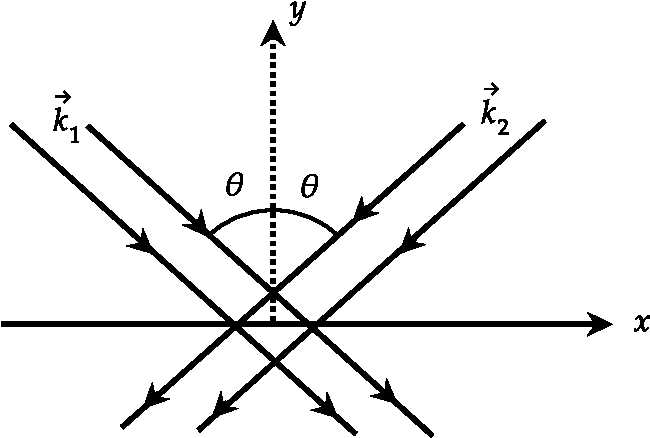
\includegraphics[height=3.3cm,width=5cm]{Net-19-18}
\end{figure}
If the angle $\theta$ is $30^{\circ}$, the fringe spacing of the interference pattern produced on the plane is
 \begin{tasks}(2)
	\task[\textbf{a.}]$1.0 \mu m$
	\task[\textbf{b.}]$0.29 \mu \mathrm{m}$
	\task[\textbf{c.}]$0.58 \mu \mathrm{m}$
	\task[\textbf{d.}]$0.5 \mu m$ 
\end{tasks}
\item  Which of the following is not a correct boundary condition at an interface between two homogeneous dielectric media? (In the following $\hat{n}$ is a unit vector normal to the interface, $\sigma$ and $\vec{j}_{s}$, are the surface charge and current densities, respectively.)
 \begin{tasks}(2)
	\task[\textbf{a.}]$\hat{n} \times\left(\vec{D}_{1}-\vec{D}_{2}\right)=0$
	\task[\textbf{b.}] $\hat{n} \times\left(\vec{H}_{1}-\vec{H}_{2}\right)=\vec{j}_{s}$
	\task[\textbf{c.}]$\hat{n} \cdot\left(\vec{D}_{1}-\vec{D}_{2}\right)=\sigma$
	\task[\textbf{d.}]  $\hat{n} \cdot\left(\vec{B}_{1}-\vec{B}_{2}\right)=0$
\end{tasks}
\item The permittivity tensor of a uniaxial anisotropic medium, in the standard Cartesian basis, is $\left(\begin{array}{ccc}4 \varepsilon_{0} & 0 & 0 \\ 0 & 4 \varepsilon_{0} & 0 \\ 0 & 0 & 9 \varepsilon_{0}\end{array}\right)$ where $\varepsilon_{0}$ is a constant. The wave number of an electromagnetic plane wave polarized along the $x$-direction, and propagating along the $y$-direction in this medium (in terms of the wave number $k_{0}$ of the wave in vacuum) is
 \begin{tasks}(2)
	\task[\textbf{a.}] $4 k_{0}$
	\task[\textbf{b.}]$2 k_{0}$
	\task[\textbf{c.}] $9 k_{0}$
	\task[\textbf{d.}] $3 k_{0}$
\end{tasks}
\item  The element of a $3 \times 3$ matrix $A$ are the products if its row and column indices $A_{i j}=i j$ (where $i, j=1,2,3$ ). The eigenvalues of $A$ are
 \begin{tasks}(2)
	\task[\textbf{a.}]$(7,7,0)$
	\task[\textbf{b.}]$(7,4,3)$
	\task[\textbf{c.}]$(14,0,0)$
	\task[\textbf{d.}] $\left(\frac{14}{3}, \frac{14}{3}, \frac{14}{3}\right)$
\end{tasks}
\item In the following circuit, each device $D$ may be an insulator with probability $p$ or a conductor with probability $(1-p)$.
\begin{figure}[H]
	\centering
	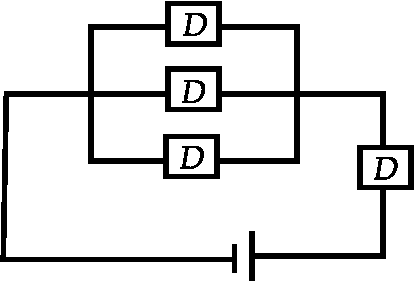
\includegraphics[height=2.5cm,width=4cm]{Net-19-19}
\end{figure}
The probability that a non-zero current flows through the circuit is
 \begin{tasks}(2)
	\task[\textbf{a.}] $2-p-p^{3}$
	\task[\textbf{b.}] $(1-p)^{4}$
	\task[\textbf{c.}] $(1-p)^{2} p^{2}$
	\task[\textbf{d.}] $(1-p)\left(1-p^{3}\right)$
\end{tasks}
\item The solution of the differential equation $x \frac{d y}{d x}+(1+x) y=e^{-x}$ with the boundary condition $y(x=1)=0$, is
 \begin{tasks}(2)
	\task[\textbf{a.}]$\frac{(x-1)}{x} e^{-x}$
	\task[\textbf{b.}] $\frac{(x-1)}{x^{2}} e^{-x}$
	\task[\textbf{c.}] $\frac{(1-x)}{x^{2}} e^{-x}$
	\task[\textbf{d.}] $(x-1)^{2} e^{-x}$
\end{tasks}
\item The value of the definite integral $\int_{0}^{\pi} \frac{d \theta}{5+4 \cos \theta}$ is
 \begin{tasks}(2)
	\task[\textbf{a.}]$\frac{4 \pi}{3}$
	\task[\textbf{b.}] $\frac{2 \pi}{3}$
	\task[\textbf{c.}]$\pi$
	\task[\textbf{d.}]$\frac{\pi}{3}$ 
\end{tasks}
\item In a system comprising of approximately $10^{23}$ distinguishable particles, each particle may occupy any of 20 distinct states. The maximum value of the entropy per particle is nearest to
 \begin{tasks}(2)
	\task[\textbf{a.}] $20 k_{B}$
	\task[\textbf{b.}]$3 k_{B}$
	\task[\textbf{c.}]$10(\ln 2) k_{B}$
	\task[\textbf{d.}]$20(\ln 2) k_{B}$ 
\end{tasks}
\item  Consider a classical gas in thermal equilibrium at temperatures $T_{1}$ and $T_{2}$ where $T_{1}<T_{2}$. Which of the following graphs correctly represents the qualitative behaviour of the probability density function of the $x$-component of the velocity?
 \begin{tasks}(2)
	\task[\textbf{a.}]
	\begin{figure}[H]
		\centering
		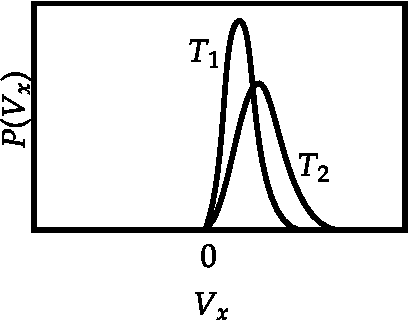
\includegraphics[height=2.5cm,width=3.5cm]{Net-19-20}
	\end{figure}
	\task[\textbf{b.}]
		\begin{figure}[H]
		\centering
		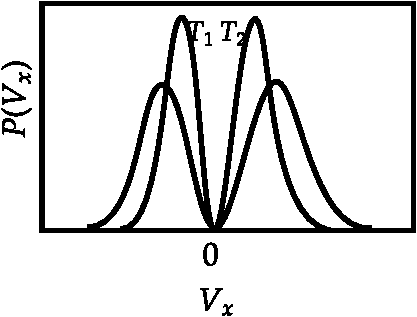
\includegraphics[height=2.5cm,width=3.5cm]{Net-19-21}
	\end{figure}
	\task[\textbf{c.}]
		\begin{figure}[H]
		\centering
		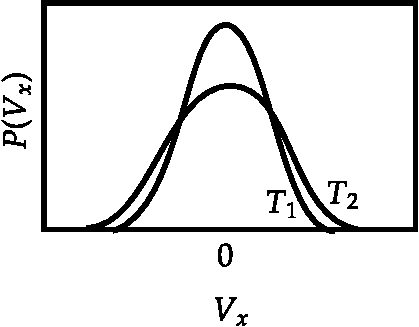
\includegraphics[height=2.5cm,width=3.5cm]{Net-19-22}
	\end{figure}
	\task[\textbf{d.}] 
		\begin{figure}[H]
		\centering
		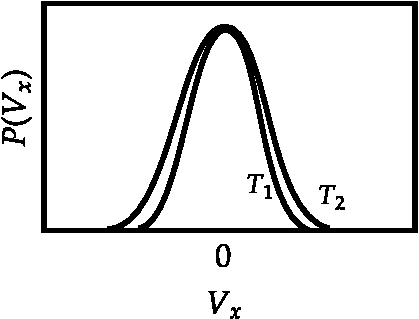
\includegraphics[height=2.5cm,width=3.5cm]{Net-19-23}
	\end{figure}
\end{tasks}
\item  The equation of state of an ideal gas is $p V=R T .$ At very low temperatures, the volume expansion coefficient $\frac{1}{V} \frac{\partial V}{\partial T}$ at constant pressure
 \begin{tasks}(2)
	\task[\textbf{a.}]Diverges as $\frac{1}{T^{2}}$
	\task[\textbf{b.}]Diverges as $\frac{1}{T}$
	\task[\textbf{c.}]Vanishes as $T$
	\task[\textbf{d.}]Is independent of the temperature 
\end{tasks}
\item  The Hamiltonian of a classical nonlinear one dimensional oscillator is $H=\frac{1}{2 m} p^{2}+\lambda x^{4}$, where $\lambda>0$ is a constant. The specific heat of a collection of a collection of $N$ independent such oscillators is
 \begin{tasks}(2)
	\task[\textbf{a.}]$\frac{3 N k_{B}}{2}$
	\task[\textbf{b.}]$\frac{3 N k_{B}}{4}$
	\task[\textbf{c.}]$N k_{B}$
	\task[\textbf{d.}]$\frac{N k_{B}}{2}$ 
\end{tasks}
\item  In an experiment to measure the acceleration due to gravity $g$ using a simple pendulum, the length and time period of the pendulum are measured to three significant figures. The mean value of $g$ and the uncertainty $\delta g$ of the measurements are then estimated using a calculator from a large number of measurements and found to be $9.82147 \mathrm{~m} / \mathrm{s}^{2}$ and $0.02357 \mathrm{~m} / \mathrm{s}^{2}$, respectively. Which of the following is the most accurate way of presenting the experimentally determined value of $g$ ?
 \begin{tasks}(2)
	\task[\textbf{a.}]$9.82 \pm 0.02 \mathrm{~m} / \mathrm{s}^{2}$
	\task[\textbf{b.}]$9.8215 \pm 0.02 \mathrm{~m} / \mathrm{s}^{2}$
	\task[\textbf{c.}]$9.82147 \pm 0.02357 \mathrm{~m} / \mathrm{s}^{2}$
	\task[\textbf{d.}] $9.82 \pm 0.02357 \mathrm{~m} / \mathrm{s}^{2}$ 
\end{tasks}
\item  An ac signal of the type as shown in the figure, is applied across a resistor $R=1 \Omega$.
\begin{figure}[H]
	\centering
	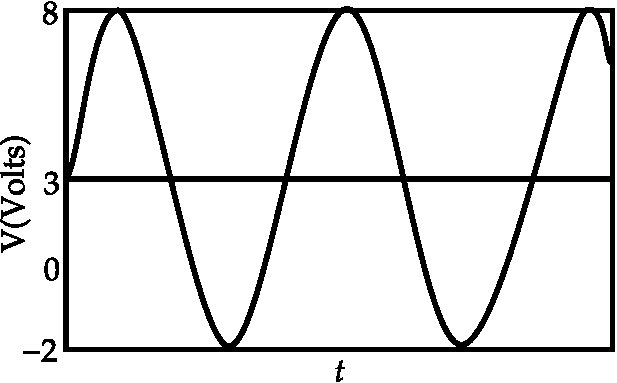
\includegraphics[height=2.5cm,width=4cm]{Net-19-24}
\end{figure}
The power dissipated across the resistor is
 \begin{tasks}(2)
	\task[\textbf{a.}]$12.5 \mathrm{~W}$
	\task[\textbf{b.}]$9 \mathrm{~W}$
	\task[\textbf{c.}]$25 \mathrm{~W}$
	\task[\textbf{d.}]$21.5 \mathrm{~W}$ 
\end{tasks}
\item  An npn-transistor is connected in a voltage divider configuration as shown in the figure below.
\begin{figure}[H]
	\centering
	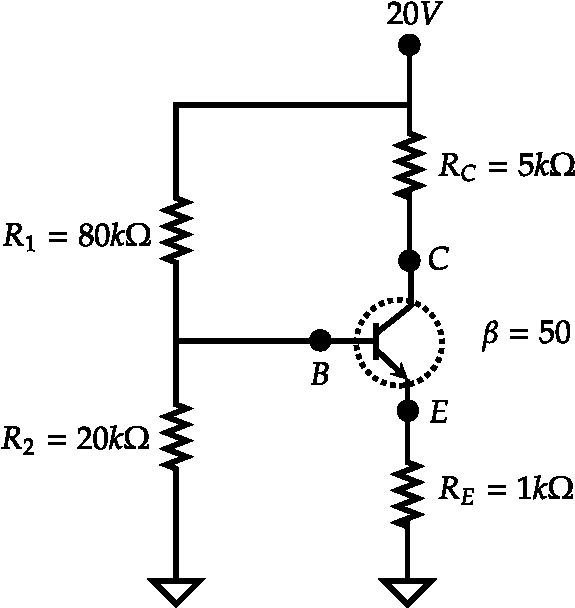
\includegraphics[height=4.3cm,width=4cm]{Net-19-25}
\end{figure}
If the resistor $R_{2}$ is disconnected, the voltages $V_{B}$ at the base and $V_{C}$ at the collector change as follows.
 \begin{tasks}(2)
	\task[\textbf{a.}]both $V_{B}$ and $V_{C}$ increase
	\task[\textbf{b.}]both $V_{B}$ and $V_{C}$ decrease
	\task[\textbf{c.}]$V_{B}$ decreases, but $V_{C}$ increases
	\task[\textbf{d.}]$V_{B}$ increases, but $V_{C}$ decreases
\end{tasks}
\item  Let $Y$ denote the output in the following logical Circuit.
\begin{figure}[H]
	\centering
	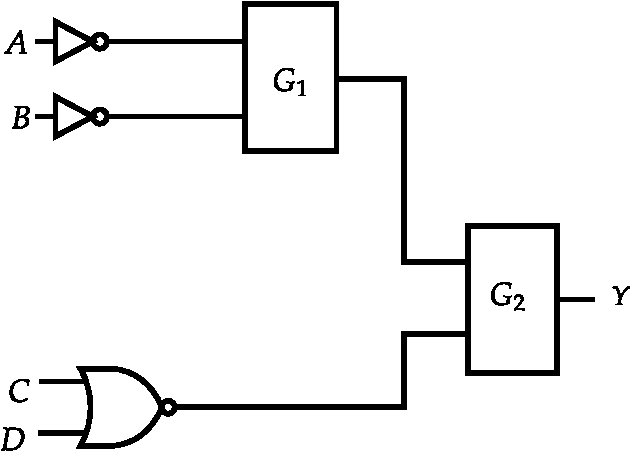
\includegraphics[height=3cm,width=4.5cm]{Net-19-26}
\end{figure}
If $Y=A B+\overline{C D}$, the gates $G_{1}$ and $G_{2}$ must, respectively, be
 \begin{tasks}(2)
	\task[\textbf{a.}]OR and NAND
	\task[\textbf{b.}]NOR and $\mathrm{OR}$
	\task[\textbf{c.}] AND and NAND
	\task[\textbf{d.}]  NAND and OR
\end{tasks}
\item  A solid spherical Cork of radius $R$ and specific gravity $0.5$ floats on water. The cork is pushed down so that its Centre of mass is at a distance $h$ (where $0<h<R$ ) below the surface of water, and Then released. The volume of the part of the cork above water level is $\pi R^{3}\left(\frac{2}{3}-\cos \theta_{0}+\frac{1}{3} \cos ^{3} \theta_{0}\right)$ where $\theta_{0}$ is the angle as shown in the figure.
\begin{figure}[H]
	\centering
	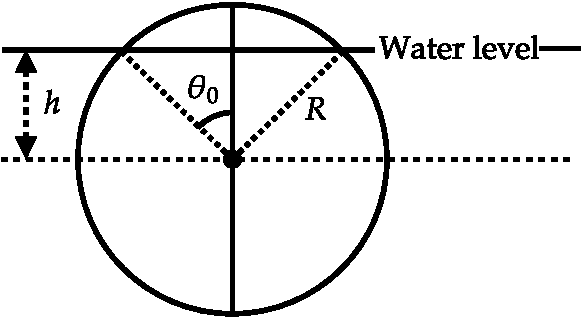
\includegraphics[height=2.7cm,width=5cm]{Net-19-27}
\end{figure}
At the moment of release, the dependence of the upward force on the cork on $h$ is
 \begin{tasks}(2)
	\task[\textbf{a.}]$\frac{h}{R}-\frac{1}{3}\left(\frac{h}{R}\right)^{3}$
	\task[\textbf{b.}]$\frac{h}{R}+\frac{1}{3}\left(\frac{h}{R}\right)^{3}$
	\task[\textbf{c.}]$\frac{h}{R}-\frac{2}{3}\left(\frac{h}{R}\right)^{3}$
	\task[\textbf{d.}] $\frac{h}{R}+\frac{2}{3}\left(\frac{h}{R}\right)^{3}$
\end{tasks}
\item Two particles of masses $m_{1}$ and $m_{2}$ are connected by a massless thread of length $l$ as shown in figure below.
\begin{figure}[H]
	\centering
	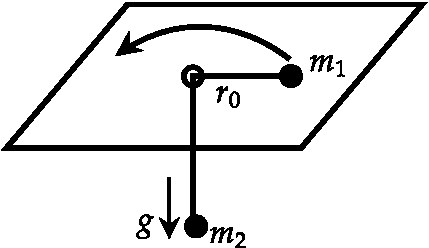
\includegraphics[height=2cm,width=4cm]{Net-19-28}
\end{figure}
The particle of mass in on the plane undergoes a circular motion with radius $r_{0}$ and angular momentum $L$. When a small radial displacement $\in$ (whew $\in<<r_{0}$ ) is applied, its radial coordinate is found to oscillate about $r_{0}$. The frequency of the oscillations is
 \begin{tasks}(2)
	\task[\textbf{a.}] $\sqrt{\frac{7 m_{2} g}{\left(m_{1}+\frac{m_{2}}{2}\right) r_{0}}}$
	\task[\textbf{b.}]$\sqrt{\frac{7 m_{2} g}{\left(m_{1}+m_{2}\right) r_{0}}}$
	\task[\textbf{c.}]$\sqrt{\frac{3 m_{2} g}{\left(m_{1}+\frac{m_{2}}{2}\right) r_{0}}}$
	\task[\textbf{d.}] $\sqrt{\frac{3 m_{2} g}{\left(m_{1}+m_{2}\right) r_{0}}}$
\end{tasks}
\item  The time evolution of a coordinate $x$ of a particle is described by the equation
$$
\frac{d^{2} x}{d t^{4}}+2 \Omega^{2} \frac{d^{2} x}{d t^{2}}+\left(\Omega^{4}-A^{4}\right) x=0
$$
For $\Omega>A$, the particle will
 \begin{tasks}(2)
	\task[\textbf{a.}]Eventually come to rest at the origin
	\task[\textbf{b.}] Eventually drift to infinity $(|x| \rightarrow \infty)$
	\task[\textbf{c.}] Oscillate about the origin
	\task[\textbf{d.}] Eventually come to rest at $\frac{\Omega}{A}$ or $-\frac{\Omega}{A}$
\end{tasks}
\item  The Hamiltonian of a quantum particle of mass $m$ is $H=\frac{p^{2}}{2 m}+\alpha|x|^{r}$, where $\alpha$ and $r$ are positive constants. The energy $E_{n}$ of the $n^{t h}$ level for large $n$, depends on $n$ as
 \begin{tasks}(2)
	\task[\textbf{a.}]$n^{2 r}$
	\task[\textbf{b.}]$n^{r+2}$
	\task[\textbf{c.}]$n^{1 /(r+2)}$
	\task[\textbf{d.}] $n^{2 r /(r+2)}$
\end{tasks}
\item In the partial wave expansion, the differential scattering cross-section is given by
$$
\frac{d \sigma}{d(\cos \theta)}=\left|\sum_{l}(2 l+1) e^{i \delta_{i}} \sin \delta_{l} P_{l}(\cos \theta)\right|^{2}
$$
where $\theta$ is the scattering angle. For a certain neutron-nucleus scattering. It is found that the two lowest phase shifts $\delta_{0}$ and $\delta_{1}$ corresponding to $s$-wave and $p$-wave, respectively, satisfy $\delta_{1} \approx \frac{\delta_{0}}{2}$. Assuming that the other phase shifts are negligibly small, the differential cross-section reaches its minimum for $\cos \theta$ equal to
 \begin{tasks}(2)
	\task[\textbf{a.}]0
	\task[\textbf{b.}] $\pm 1$
	\task[\textbf{c.}]$-\frac{2}{3} \cos ^{2} \delta_{1}$
	\task[\textbf{d.}]  $\frac{1}{3} \cos ^{2} \delta_{1}$
\end{tasks}
\item A charged, spin-less particle of mass $m$ is subjected to an attractive potential $V(x, y, z)=\frac{1}{2} k\left(x^{2}+y^{2}+z^{2}\right)$, where $k$ is a positive constant. Now a perturbation in the form of a weak magnetic field $B=B_{0} \hat{k}$ (where $B_{0}$ is a constant) is switched on. Into how many distinct levels will the second excited state of the unperturbed Hamiltonian split?
 \begin{tasks}(2)
	\task[\textbf{a.}]5
	\task[\textbf{b.}]4
	\task[\textbf{c.}]2
	\task[\textbf{d.}] 1
\end{tasks}
\item  The elastic scattering of a charged particle of mass $m$ off an atom can be approximated by the potential $V(r)=\frac{\alpha}{r} e^{-r / R}$ where $\alpha$ and $R$ are positive constants.\\
If the wave number of the incoming particle is $k$ and the scattering angle is $2 \theta$, the differential cross-section in the Born approximation is
 \begin{tasks}(2)
	\task[\textbf{a.}]$\frac{m^{2} \alpha^{2} R^{4}}{4 \hbar^{4}\left(1+k^{3} R^{2} \sin ^{2} \theta\right)}$
	\task[\textbf{b.}]$\frac{m^{2} \alpha^{2} R^{4}}{\hbar^{4}\left(2 k^{2} R^{2} \sin ^{2} \theta\right)^{2}}$
	\task[\textbf{c.}] $\frac{2 m^{2} \alpha^{2} R^{4}}{\hbar^{4}\left(2 k^{2} R^{2} 2 \sin ^{2} \theta\right)}$
	\task[\textbf{d.}] $\frac{4 m^{2} \alpha^{2} R^{4}}{\hbar^{4}\left(1+4 k^{2} R^{2} \sin ^{2} \theta\right)^{2}}$
\end{tasks}
\item  The wave number $k$ and the angular frequency $\omega$ of a wave are related by the dispersion relation $\omega^{2}=\alpha k+\beta k^{3}$ where $\alpha$ and $\beta$ are positive constants. The wave number for which the phase velocity equals the group velocity, is
 \begin{tasks}(2)
	\task[\textbf{a.}]$3 \sqrt{\frac{\alpha}{\beta}}$
	\task[\textbf{b.}]$\sqrt{\frac{\alpha}{\beta}}$
	\task[\textbf{c.}]$\frac{1}{2} \sqrt{\frac{\alpha}{\beta}}$
	\task[\textbf{d.}] $\frac{1}{3} \sqrt{\frac{\alpha}{\beta}}$
\end{tasks}
\item  A inertial observer $A$ at rest measures the electric and magnetic field $E=(\alpha, 0,0)$ and $B=(\alpha, 0,2 \alpha)$ in a region, where a is a constant. Another inertial observer $B$, moving with a constant velocity with respect to $A$, measures the fields as $E^{\prime}=\left(E_{x}^{\prime}, \alpha, 0\right)$ and $B^{\prime}=\left(\alpha, B_{y}^{\prime}, \alpha\right)$. Then in units $c=1, E_{x}^{\prime}$ and $B_{y}^{\prime}$ are given, respectively, by
 \begin{tasks}(2)
	\task[\textbf{a.}]$-2 \alpha$ and $\alpha$
	\task[\textbf{b.}] $2 \alpha$ and $-\alpha$
	\task[\textbf{c.}] $\alpha$ and $-2 \alpha$
	\task[\textbf{d.}] $-\alpha$ and $2 \alpha$
\end{tasks}
\item  A point charge is moving with a uniform velocity $\beta C$ along the positive $x$-direction, parallel to and very close to a corrugated metal sheet (see the figure below).
\begin{figure}[H]
	\centering
	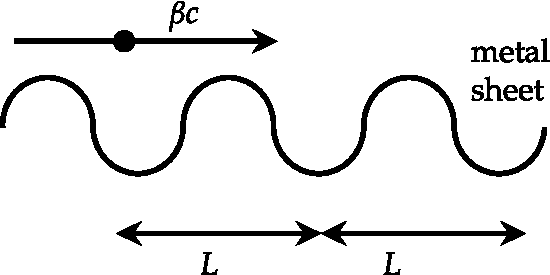
\includegraphics[height=2cm,width=4cm]{Net-19-29}
\end{figure}
The wavelength of the electromagnetic radiation received by an observer along the direction of motion is
 \begin{tasks}(2)
	\task[\textbf{a.}]$\frac{1}{\beta} \sqrt{1-\beta^{2}}$
	\task[\textbf{b.}]$L \sqrt{1-\beta^{2}}$
	\task[\textbf{c.}]$L \beta \sqrt{1-\beta^{2}}$
	\task[\textbf{d.}] $L$
\end{tasks}
\item If the Newton-Raphson method is used to find the positive root of the equation $x=2 \sin x$, the iteration equation is
 \begin{tasks}(2)
	\task[\textbf{a.}]$x_{n+1}=\frac{2 x_{n}-2\left(\sin x_{n}+x_{n} \cos x_{n}\right)}{1-2 \cos x_{n}}$
	\task[\textbf{b.}]$x_{n+1}=\frac{2\left(\sin x_{n}-x_{n} \cos x_{n}\right)}{1-2 \cos x_{n}}$
	\task[\textbf{c.}] $x_{n+1}=\frac{x_{n}^{2}-1+2\left(\cos x_{n}-x_{n} \sin x_{n}\right)}{x_{n}-2 \sin x_{n}}$
	\task[\textbf{d.}]  $x_{n+1}=\frac{x_{n}^{2}-1-2\left(\cos x_{n}+\sin x_{n}\right)}{x_{n}-2 \sin x_{n}}$
\end{tasks}
\item  The equation of motion of a forced simple harmonic oscillator is $\ddot{x}+\omega^{2} x=A \cos \Omega t$, where $A$ is a constant. At resonance $\Omega=\omega$ the amplitude of oscillations at large times
 \begin{tasks}(2)
	\task[\textbf{a.}]saturates to a finite value
	\task[\textbf{b.}] increases with time as $\sqrt{t}$
	\task[\textbf{c.}] increases linearly with time
	\task[\textbf{d.}]  increases exponentially with time
\end{tasks}
\item The operator $A$ has a matrix representation $\left(\begin{array}{ll}2 & 1 \\ 1 & 2\end{array}\right)$ in the basis spanned by $\left(\begin{array}{l}1 \\ 0\end{array}\right)$ and $\left(\begin{array}{l}0 \\ 1\end{array}\right)$. In another basis spanned by $\frac{1}{\sqrt{2}}\left(\begin{array}{l}1 \\ 1\end{array}\right)$ and $\frac{1}{\sqrt{2}}\left(\begin{array}{c}1 \\ -1\end{array}\right)$, the matrix representation of $A$ is
 \begin{tasks}(2)
	\task[\textbf{a.}]$\left(\begin{array}{ll}2 & 0 \\ 0 & 2\end{array}\right)$
	\task[\textbf{b.}]$\left(\begin{array}{ll}3 & 0 \\ 0 & 1\end{array}\right)$
	\task[\textbf{c.}]$\left(\begin{array}{ll}3 & 1 \\ 0 & 1\end{array}\right)$
	\task[\textbf{d.}] $\left(\begin{array}{ll}3 & 0 \\ 1 & 1\end{array}\right)$
\end{tasks}
\item The operator $x \frac{d}{d x} \delta(x)$, where $\delta(x)$ is the Dirac delta function, acts on the space of real -valued square-integrable functions on the real line. This operator is equivalent to
 \begin{tasks}(2)
	\task[\textbf{a.}]$-\delta(x)$
	\task[\textbf{b.}]$\delta(x)$
	\task[\textbf{c.}]$x$
	\task[\textbf{d.}]0
\end{tasks}
\item At each time step, a random walker in one dimension either remains at the same point with probability $\frac{1}{4}$, or moves by a distance $\Delta$ to the right or left with probabilities $\frac{3}{8}$ each. After $N$ time steps, its root mean squared displacement is
 \begin{tasks}(2)
	\task[\textbf{a.}]$\Delta \sqrt{N}$
	\task[\textbf{b.}] $\Delta \sqrt{\frac{9 N}{16}}$
	\task[\textbf{c.}]$\Delta \sqrt{\frac{3 N}{4}}$
	\task[\textbf{d.}] $\Delta \sqrt{\frac{3 N}{8}}$
\end{tasks}
\item The Hamiltonian of three Ising spins $S_{1}, S_{2}$ and $S_{3}$, each taking values $\pm 1$, is $H=-J\left(S_{1} S_{2}+S_{2} S_{3}\right)-h S_{1}$, where $J$ and $h$ are positive constants. The mean value of $S_{3}$ in equilibrium at a temperature $T=1 /\left(k_{B} \beta\right)$, is
 \begin{tasks}(2)
	\task[\textbf{a.}]$\tanh ^{3}(\beta J)$
	\task[\textbf{b.}]$\tan (\beta h) \tanh ^{2}(\beta J)$
	\task[\textbf{c.}]$\sinh (\beta h) \sinh ^{2}(\beta J)$
	\task[\textbf{d.}] 0
\end{tasks}
\item The free energy of a magnetic system, as a function of its magnetisation $m$, is $F=\frac{1}{2} a m^{2}-\frac{1}{4} b m^{4}+\frac{1}{6} m^{6}$. where $a$ and $b$ are positive constants $.$

At a fixed value of $a$, the critical value of $b$, above which the minimum of $F$ will be at a non-zero value of magnetisation, is
 \begin{tasks}(2)
	\task[\textbf{a.}]$\sqrt{\frac{10 a}{3}}$
	\task[\textbf{b.}]$\sqrt{\frac{16 a}{3}}$
	\task[\textbf{c.}] $\frac{10}{3} \sqrt{a}$
	\task[\textbf{d.}] $\frac{16}{3} \sqrt{a}$
\end{tasks}
\item For optimal performance of an op-amp based current-to-voltage converter circuit, the input and output impedance should be
 \begin{tasks}(2)
	\task[\textbf{a.}] Low input impedance and high output impedance
	\task[\textbf{b.}]Low input impedance and low output impedance
	\task[\textbf{c.}] High input impedance and high output impedance
	\task[\textbf{d.}] High input impedance and low output impedance
\end{tasks}
\item The forward diode current is given by $I=k T^{\alpha} e^{-E_{g} / k_{B} T}\left(\exp \left(e V / k_{B} T\right)-1\right)$, where $E_{g}$ is the band gap of the semiconductor, $V$ is the voltage drop across the diode, $T$ is the temperature of the diode operating near room temperature and, $\alpha$ and $K$ are constants. A diode is used as a thermal sensor in the circuit shown below.
\begin{figure}[H]
	\centering
	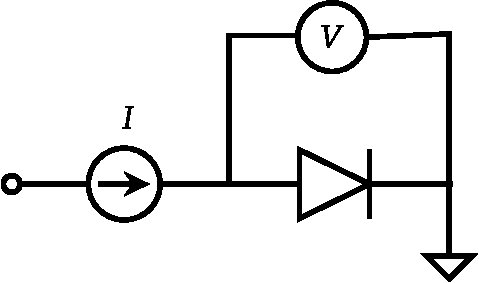
\includegraphics[height=2cm,width=3.5cm]{Net-19-30}
\end{figure}
If $V$ is measured using an ideal voltmeter to estimate $T$, the variation of the voltage $V$ as a function of $T$ is best approximated by (in the following $a$ and $b$ are constants)
 \begin{tasks}(2)
	\task[\textbf{a.}] $a T^{2}+b$
	\task[\textbf{b.}] $a T+b$
	\task[\textbf{c.}] $a T^{3}+b$
	\task[\textbf{d.}] $a T+b T^{2}$
\end{tasks}
\item A circuit constructed using op-amp, resistor $R_{1}=1 k \Omega$ and capacitors $C_{1}=1 \mu F$ and $C_{2}=0.1 \mu F$ is shown in the figure below.
\begin{figure}[H]
	\centering
	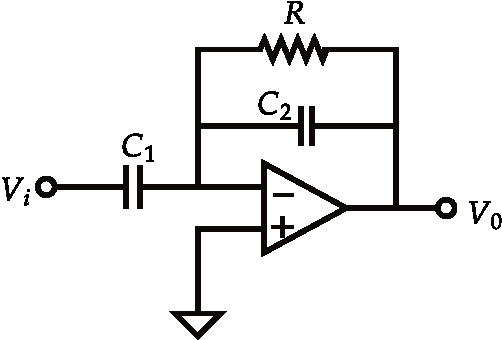
\includegraphics[height=3cm,width=4.5cm]{Net-19-31}
\end{figure}
This circuit will act as a
 \begin{tasks}(2)
	\task[\textbf{a.}]High pass filter
	\task[\textbf{b.}]Low pass filter
	\task[\textbf{c.}]Band pass filter
	\task[\textbf{d.}]Band reject filter 
\end{tasks}
\item The third-nearest neighbour distance in a BCC (Body Centered Cubic) crystal with lattice constant $a_{0}$ is
 \begin{tasks}(2)
	\task[\textbf{a.}] $a_{0}$
	\task[\textbf{b.}]$\frac{3 a_{0}}{2}$
	\task[\textbf{c.}] $\sqrt{3} a_{0}$
	\task[\textbf{d.}]  $\sqrt{2} a_{0}$
\end{tasks}
\item A bound electron and hole pair interacting via Coulomb interaction in a semiconductor is called an exciton. The effective masses of an electron and a hole are about $0.1 m_{e}$ and $0.5 m_{e}$ respectively, where $m_{e}$ is the rest mass of the electron. The dielectric constant of the semiconductor is 10 . Assuming that the energy levels of the excitons are hydrogenlike, the binding energy of an exciton (in units of the Rydberg constant) is closest to
 \begin{tasks}(2)
	\task[\textbf{a.}]$2 \times 10^{-3}$
	\task[\textbf{b.}]$2 \times 10^{-4}$
	\task[\textbf{c.}]$8 \times 10^{-4}$
	\task[\textbf{d.}]$3 \times 10^{-3}$ 
\end{tasks}
\item Consider an array of atoms in one dimension with an ensemble averaged periodic density distribution as shown in the figure.
\begin{figure}[H]
	\centering
	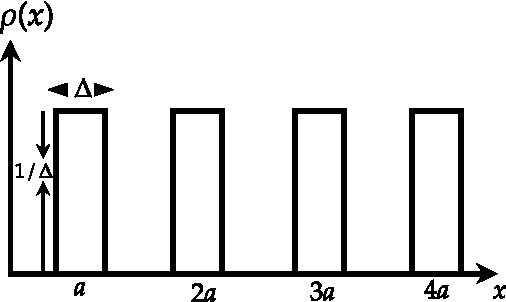
\includegraphics[height=3cm,width=5cm]{Net-19-32}
\end{figure}
If $k$ is the wave number and $S(k, \Delta)$ denotes the Fourier transform of the densitydensity correlation function, the ratio $\frac{S(k, \Delta)}{S(k, 0)}$ is
 \begin{tasks}(2)
	\task[\textbf{a.}] $\cos \left(\frac{k \Delta}{2}\right)$
	\task[\textbf{b.}] $\cos ^{2}\left(\frac{k \Delta}{2}\right)$
	\task[\textbf{c.}] $\frac{2}{k \Delta} \sin \left(\frac{k \Delta}{2}\right)$
	\task[\textbf{d.}] $\frac{4}{k^{2} \Delta^{2}} \sin ^{2}\left(\frac{k \Delta}{2}\right)$
\end{tasks}
\item A doubly charged ion in the angular momentum state $\left(J=2, J_{3}=1\right)$ meets a gas of polarized electrons $\left(S_{3}=\frac{1}{2}\right)$ and gets neutralized. If the orbital angular momentum transferred in the process is zero, the probability that the neutral atom is in the $\left(J=2, J_{3}=2\right)$ state is
 \begin{tasks}(2)
	\task[\textbf{a.}] $\frac{2}{5}$
	\task[\textbf{b.}]$\frac{2}{3}$
	\task[\textbf{c.}]$\frac{1}{5}$
	\task[\textbf{d.}] $\frac{1}{3}$
\end{tasks}
\item The range of the inter-atomic potential in gaseous hydrogen is approximately $5 \AA \AA^{\circ}$ In thermal equilibrium, the maximum temperature for which the atom-atom scattering is dominantly $s$-wave, is
 \begin{tasks}(2)
	\task[\textbf{a.}]$500 \mathrm{~K}$
	\task[\textbf{b.}]$100 \mathrm{~K}$
	\task[\textbf{c.}] $1 K$
	\task[\textbf{d.}] $1 m K$
\end{tasks}
\item The energy levels corresponding to the rotational motion of a molecule are $E_{J}=B J(J+1) \mathrm{cm}^{-1}$ where $J=0,1,2, \ldots$, and $B$ is a constant. Pure rotational Raman transitions follow the selection rule $\Delta J=0, \pm 2$. When the molecule is irradiated, the separation between the closest Stokes and anti-Stokes lines (in $\mathrm{cm}^{-1}$ ) is
 \begin{tasks}(2)
	\task[\textbf{a.}] $6 B$
	\task[\textbf{b.}]$12 B$
	\task[\textbf{c.}]$4 B$
	\task[\textbf{d.}]$8 B$ 
\end{tasks}
\item The cavity of a He-Ne laser emitting at $632.8 \mathrm{~nm}$, consists of two mirrors separated by a distance of $35 \mathrm{~cm}$. If the oscillations in the laser cavity occur at frequencies within the gain bandwidth of $1.3 \mathrm{GHz}$, the number of longitudinal modes allowed in the cavity is
 \begin{tasks}(2)
	\task[\textbf{a.}]1
	\task[\textbf{b.}]2
	\task[\textbf{c.}]3
	\task[\textbf{d.}] 4
\end{tasks}
\item An excited state of a ${ }_{4}^{8}$ Be nucleus decays into two $\alpha$-particles which are in a spinparity $0^{+}$state. If the mean life-time of this decay is $10^{-22} s$, the spin-parity of the excited state of the nucleus is
 \begin{tasks}(2)
	\task[\textbf{a.}]$2^{+}$
	\task[\textbf{b.}]$3^{+}$
	\task[\textbf{c.}]$0^{-}$
	\task[\textbf{d.}]$4^{-}$ 
\end{tasks}
\item The elastic scattering of a neutrino $v_{e}$ by an electron $e^{-}$, i.e. the reaction $v_{e}+e^{-} \rightarrow v_{e}+e^{-}$can be described by the interaction Hamiltonian
$$
H_{\text {int }}=\frac{1}{\sqrt{2}} G_{F} \int d^{3} x\left(\bar{\psi}_{e}(x) \gamma^{\mu} \psi_{v e}(x)\right)\left(\bar{\psi}_{v e}(x) \gamma_{\mu} \psi_{e}(x)\right)
$$
The cross-section of the above process depends on the centre of mass energy $E$, as
 \begin{tasks}(2)
	\task[\textbf{a.}]$\frac{1}{E^{2}}$
	\task[\textbf{b.}]$E^{2}$
	\task[\textbf{c.}]$E$
	\task[\textbf{d.}]$\sqrt{E}$ 
\end{tasks}
\item  The mean life-time of the following decays:\\
$\rho_{0} \rightarrow \pi^{+}+\pi^{-}, \pi^{0} \rightarrow \gamma+\gamma, \mu^{-} \rightarrow e^{-}+\bar{v}_{e}+v_{\mu}$, are $\tau_{\rho}, \tau_{\pi}$ and $\tau_{\mu}$ respectively.
They satisfy
 \begin{tasks}(2)
	\task[\textbf{a.}]$\tau_{\pi}<\tau_{\rho}<\tau_{\mu}$
	\task[\textbf{b.}]$\tau_{\mu}<\tau_{\rho}<\tau_{\pi}$
	\task[\textbf{c.}]$\tau_{\rho}<\tau_{\pi}<\tau_{\mu}$
	\task[\textbf{d.}]$\tau_{\rho}<\tau_{\mu}<\tau_{\pi}$ 
\end{tasks}
\end{enumerate}